\section{Detection Pipeline}
\label{sec:pipeline}

\subsection{Overview}

Figure~\ref{fig:overview} presents the two phases of \tool. The offline phase
constructs the obligation specification described in
Section~\ref{sec:construction}. The online phase consumes a native-extension
project and produces auditable bug reports. Static analysis first discovers
candidate functions, binds API calls to obligations, and prunes obligation
instances using syntactic patterns. Structured LLM checking then
tests every retained obligation against its discharge conditions. Only
high-confidence violated judgments become reports.

\begin{figure*}[t]
\centering
\begin{tikzpicture}
  \node[anchor=south west,inner sep=0] (overview) at (0,0) {
    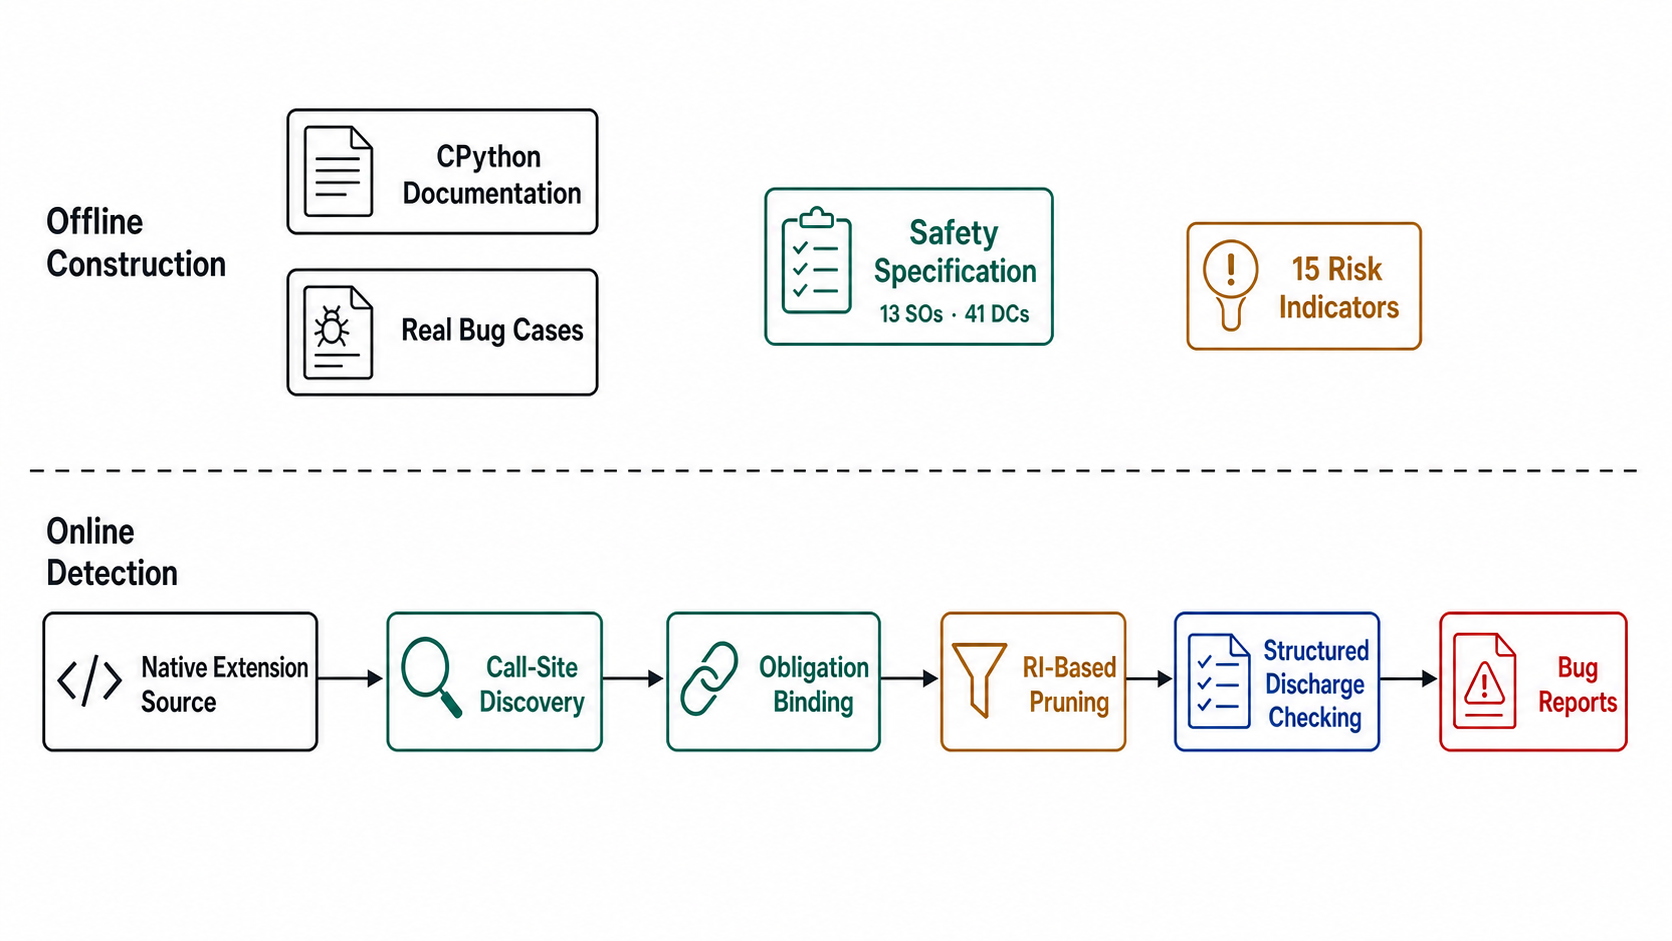
\includegraphics[width=0.90\textwidth]{figures/pycguard_overview.png}
  };
  \begin{scope}[x={(overview.south east)},y={(overview.north west)}]
    \tikzset{flow/.style={->,>=stealth,line width=0.55pt,draw=black!80,
                          rounded corners=1pt}}
    % Evidence sources to offline artifacts.
    \draw[flow] (0.355,0.82) -| (0.455,0.72);
    \draw[flow] (0.355,0.64) -| (0.455,0.68);
    % Static pruning owns these patterns; mask the obsolete offline RI box.
    \fill[white] (0.70,0.60) rectangle (0.87,0.80);
    % Offline artifacts to their only online consumers.
    \draw[flow] (0.505,0.61) -- (0.505,0.40) -- (0.465,0.40)
                -- (0.465,0.33);
    \draw[flow] (0.590,0.61) -- (0.590,0.39) -- (0.765,0.39)
                -- (0.765,0.33);
  \end{scope}
\end{tikzpicture}
\caption{PyCGuard workflow. Safety obligations and discharge conditions define
the checked properties. Static pattern matching prunes bound instances before
LLM checking.}
\label{fig:overview}
\end{figure*}

The pipeline uses the function as its context unit and a pair $(f,o)$ as its
checking unit. Grouping calls by function preserves cleanup labels and branch
conditions shared by several API calls. Separating obligations prevents one
large prompt from asking the model to discover arbitrary defects. A function
can therefore produce several checking units before pruning, each with one
property and a small set of discharge alternatives.

\subsection{Candidate Generation}

\paragraph{Source discovery.}
The scanner walks C and C++ source and header files. A file is selected when it
directly includes \code{Python.h} or contains Python/C API symbols. The second
criterion covers indirect includes and generated wrappers. Header files are
recorded because inline extension code can reside in headers, although the
evaluation reports source-file coverage separately.

\paragraph{Call-site discovery.}
Tree-sitter parses each selected file and identifies call expressions and their
enclosing function definitions. The current specification indexes 147 API
names. Calls outside a function are ignored because the checker requires an
enclosing control-flow context. Parse errors are retained as metadata so that
malformed or dialect-specific input can be audited.

\paragraph{Obligation binding.}
For each indexed call, \tool retrieves all associated SOs and records the API,
arguments, location, and obligation category. It extracts the subject from the
left-hand side for object-producing APIs, from the consumed argument for
steal-reference APIs, and from the first argument for decrement operations.
All trigger sites in the same function are aggregated. Repeated calls at the
same location are deduplicated, and the union of bound SOs forms the unpruned
candidate.

\paragraph{Local use facts.}
The analyzer traverses the enclosing syntax tree for references to each
trigger variable. It classifies simple assignments, null checks, decrement
calls, ownership-consuming calls, returns, and other uses. It also follows
simple local aliases. These facts support static pattern matching; they are not
used to establish a final safe verdict.

\subsection{Static Pattern-Based Pruning}

The pruning module defines 15 risk-indicator patterns for eight SO categories;
they are analyzer rules rather than fields in the obligation specification.
The module maintains a registry from an SO identifier to an executable pattern
checker. Each checker consumes the trigger sites, the local-use facts collected
for trigger variables, and the enclosing function text. This organization
keeps pattern evolution independent of the JSON specification: adding or
weakening a screen changes candidate selection but not the property sent to the
LLM.

The patterns fall into three operational groups. Ownership and lifetime
patterns look for a new reference without a release, transfer, or return; an
inline new-reference result that cannot be discharged later; borrowed-reference
use; repeated release sites; uninitialized cleanup variables; and mutation of
a reused tuple. Validation and error-state patterns detect a nullable result
whose first classified use is not a check, a callback without an exception
check, tri-state APIs treated as booleans, and APIs that suppress exceptions.
Resource and representation patterns cover unmatched allocation/release
operations, unchecked typed casts, missing write-back resolution, and narrowing
conversions. These are deliberately syntactic approximations. A matched pattern
retains an SO for checking; it never establishes a violation or replaces a DC.

For ownership, for example, the screen retains a new reference when it cannot
find a release, transfer, or return form. For null validation, it retains a
result when the first classified use after creation is not a null check. The
subsequent LLM prompt contains the SO and complete DC set, but not a claim that
the matched pattern is defective. The checker must still reason about all
relevant paths and admissible discharge alternatives.

The screen is intentionally conservative in two ways. An SO without an
implemented indicator is retained. If screening removes every SO bound to a
function, the implementation restores the original set rather than dropping
the function. This fallback prevents a candidate from disappearing solely
because the current pattern vocabulary does not describe it, although it also
limits the maximum reduction. RQ3 measures the actual reduction and checks
whether any known defect loses its $(f,o)$ pair.

\subsection{Structured Discharge Checking}

For every retained pair, the checker constructs a prompt with four components:
the SO description, its check mode, the complete DC list, and the full
enclosing function. We use the full function because exits, cleanup labels,
and ownership transfers often lie outside a local statement slice. Line
numbers, trigger sites, and variables from static analysis orient the model,
but the model must justify its decision using source evidence.

The requested procedure mirrors Equation~\ref{eq:discharge}. The model first
identifies the triggering call and subject. It then enumerates normal returns,
early returns, error jumps, and other relevant exits. For each path, it records
whether each applicable DC holds and cites variables and lines. A disjunctive
obligation is \code{SAFE} only when every listed path has at least one
satisfied DC. A conjunctive obligation requires every applicable aspect. If a
path lacks a discharge, the verdict is \code{VIOLATED} and the output names the
path and failed conditions.

The response schema contains the trigger API, subject, path list, per-condition
judgments, verdict, violation detail, and confidence. The JSON structure makes
missing paths and unsupported condition claims visible during audit. It does
not eliminate model error, which we evaluate through manual review, malformed
output, prompt ablation, and cross-model agreement.

\paragraph{Multiple triggers and exits.}
A function can contain several calls that bind the same SO. The prompt retains
all trigger sites and asks the model to identify the subject of each relevant
instance. This matters when a cleanup block releases several partially
initialized objects or when the same nullable API appears in separate
branches. The path record must connect a trigger and subject to the discharge
evidence; a decrement of another variable does not satisfy the condition.
Normal returns, error returns, cleanup jumps, and fall-through exits are all
within scope. The checker does not treat syntactic reachability as proof that a
path is feasible.

\paragraph{Check ordering.}
Retained SO identifiers are sorted before model calls. Stable ordering makes
runs easier to compare and gives the early-stop policy deterministic semantics
for a fixed model response. Early stop means that the tool reports at most the
first violated SO checked for one function in a run. The evaluation therefore
counts report units rather than claiming to enumerate every defect effect in a
function. Disabling early stop is supported for diagnostic runs that need all
SO judgments.

\paragraph{Response validation.}
The checker accepts only \code{SAFE} and \code{VIOLATED} verdicts in the
expected JSON object. Network failures are retried with increasing delays.
JSON recovery removes limited trailing-comma errors and can recover an explicit
verdict from otherwise malformed text; all other responses remain unknown.
Recovery status and raw text are preserved so that a parsed verdict does not
hide format noncompliance. RQ3 reports malformed and unknown rates separately
from detection quality.

\subsection{Report Generation}

The default checker stops after the first violated SO in a function. This
early-stop policy bounds repeated model calls and gives each report one primary
property. Report generation suppresses safe judgments, malformed outputs, and
violations below high confidence. A retained report identifies the project,
file, function, SO, trigger location, subject, violation path, and model
evidence. The high-confidence filter defines the RQ1 audit population; it does
not imply that medium- or low-confidence outputs are false.

\subsection{Implementation}

\tool is implemented in Python. The static analysis frontend uses the
Tree-sitter C and C++ grammars for parsing and AST-based pattern matching.
The obligation specification is stored as JSON, from which the tool builds
the API index and prompt fragments at load time. The pruning stage applies
AST pattern queries to filter obligation instances before any LLM call.
The LLM backend is \code{claude-sonnet-4} at temperature 0.
